\documentclass{article}
\usepackage{framed}
\usepackage{fontspec}
\usepackage{hhline}
\usepackage{hyperref}
\newcommand{\git}{\texttt{git}}
\newcommand{\Git}{\texttt{Git}}
\newcommand{\IonTorrent}{\textit{IonTorrent}}
\newcommand{\binDir}{binaries}
\newcommand{\fbinDir}{\textasciitile/\binDir}
\newcommand{\progDir}{programs}
\newcommand{\workDir}{ngs\_work}
\newcommand{\denovoDir}{denovo}
\newcommand{\reseqDir}{reseq}
\newcommand{\refSeq}{chr\_merged.fa}
\newcommand{\refDir}{ref}
\newcommand{\refFullDir}{\texttt{\textasciitile/\workDir/\reseqDir/ref}}
\newcommand{\denovo}{\textit{de-novo}}
\newcommand{\denovoReads}{readsfordenovo}
\newcommand{\dataDir}{data}
%Reference genome indexing
\newcommand{\refindex}[1]{\texttt{\fbinDir/tmap index -f #1}}
%map reads
\newcommand{\tmap}[3]{\texttt{\fbinDir/tmap map3 -f #1 \textbackslash \\
    -r #2 \textbackslash \\
    -i fastq \textbackslash \\
    -o 2 \textbackslash \\
    -s #3
  }
}
\newcommand{\tmapWithRG}[3]{\texttt{\fbinDir/tmap map3 -f #1 \textbackslash \\
    -r #2 \textbackslash \\
    -R "@RG\textbackslash tID:SomeID\textbackslash tSM:Sample1" \textbackslash \\
    -i fastq \textbackslash \\
    -o 2 \textbackslash \\
    -s #3
  }
}
\newcommand{\sortbam}[2]{\texttt{\fbinDir/samtools sort #1 \textbackslash \\ #2}}

\newcommand{\reheader}[2]{\texttt{\fbinDir/samtools view -H #1 \textbackslash \\
    | sed 's/SM:NOSM/SM:Sample1/' \textbackslash \\
    | samtools reheader - mapped\_reads.bam \textbackslash \\
    > #2
  }
}
\newcommand{\samtoolssnp}[3]{\texttt{\fbinDir/samtools mpileup -uf #1 \textbackslash \\
    #2 \textbackslash \\
    | \fbinDir/bcftools call -cv \textbackslash \\
    | \fbinDir/vcfutils.pl varFilter > #3
  }
}

\begin{document}
%\begin{titlepage}
\begin{center}
%\HRule \\
{ \huge \bfseries Commandline handling with examples on NGS data analysis \\ }

%\HRule \\
\end{center}
\end{titlepage}

\section{Basic linux commands}
Here will be briefly explained some basic linux commands.
%You don't need to memorize these, most frequently used commands w
For information about more commands, feel free to consult with the internet.

\subsection{Getting around}
\begin{tabular}{ll}
  Command & Explanation \\
  \hhline{==}
  \texttt{ls} & list contents of current directory \\
  \texttt{ls} \textit{dirname} & list contents of directory named \textit{dirname} \\
%  \textbf{cd} & \textbf{change directory} \\
  \texttt{cd} \textit{dirname} & change current directory to \textit{dirname} \\
  \texttt{cd \textasciitilde} & go to home directory (default directory) \\
  \texttt{cd ..} & go one directory up \\
  \texttt{pwd} & print name of current directory \\
  \texttt{mkdir} \textit{dirname} & make a new directory named \textit{dirname}\\
  \texttt{man} \textit{command} & show manual for \textit{command} \\
\end{tabular}

\subsection{File manipulation}
\begin{tabular}{ll}
  Command & Explanation \\
  \hhline{==}
%  cp & copy files and directories
%\textit{filename1} to \textit{filename2}
%  \textbf{cp} & \textbf{copy} \\
  \texttt{cp} \textit{filename1} \textit{filename2} & copy file \\
  \texttt{cp -r} \textit{dirname1} \textit{dirname2} & copy directory \\
  \texttt{mv} \textit{name1} \textit{name2} & move file or directory (can be used for renaming) \\
  \texttt{rm} \textit{filename} & remove file (you won't be able to recover removed file) \\
  \texttt{rm -r} \textit{dirname} & remove directory and its contents \\
  \texttt{more} \textit{filename} & command for paging through text file one screenful at a time \\
  \texttt{less} \textit{filename} & similar as more. Better for viewing large text files \\
  \texttt{cat} \textit{filename1 filename2 filenameN} & concatenate text files in print output to terminal window \\
  \texttt{head} \textit{filename} & print first 10 lines of a text file to terminal window \\
  \texttt{head -n 20} \textit{filename} &  print first 20 lines of a text file to terminal window \\
  \texttt{tail} & opposite of \texttt{head} \\
  \texttt{wc} \textit{filename} & show the number of lines, words and characters in a text file \\
  \texttt{cut -f 2} \textit{tabDelimitedFilename} & extract 2nd column from a tab delimited file \\
  \texttt{cut -f 3 -d ,} \textit{comaSeperatedFilename} & extract 3rd column from a coma seperated file \\
  \texttt{nano} \textit{filename} & open \textit{filename} in text editor \texttt{nano} \\
\end{tabular}

\subsection{Archiving and unarchiving of files}
Note that for the \texttt{tar} utility, option \texttt{c} stands for compress, 
\texttt{x} - for uncompress or extract, \texttt{z} - for dealing with tar.gz,
and \texttt{j} - for dealing with tar.bz2\\~\\
\subsubsection{Compressing}
\begin{tabular}{ll}
  Command & Explanation \\
  \hhline{==}
  \texttt{tar -cvf} \textit{filename.tar} \textit{filename} & \textbf{compress} file to \textbf{.tar} format \\
  \texttt{tar -zcvf} \textit{filename.tar.gz} \textit{filename} & \textbf{compress} file to \textbf{.tar.gz} format \\
  \texttt{tar -jcvf} \textit{filename.tar.bz2} \textit{filename} & \textbf{compress} file to \textbf{.tar.bz2} format \\
  \texttt{zip} \textit{filename.zip filename} & \textbf{compress} file to \textbf{.zip} format \\
  \texttt{gzip} \textit{filename} & \textbf{compress} file to \textbf{.gz} format \\
\end{tabular}{ll}

\subsubsection{Uncompressing}
\begin{tabular}{ll}
  Command & Explanation \\
  \hhline{==}
  \texttt{tar -xvf} \textit{filename.tar} & \textbf{uncompress} from \textbf{.tar} format \\
  \texttt{tar -zxvf} \textit{filename.tar.gz} & \textbf{uncompress} from \textbf{.tar.gz} format \\
  \texttt{tar -jxvf} \textit{filename.tar.bz2} & \textbf{uncompress} from \textbf{.tar.bz2} format \\
  \texttt{unzip} \textit{filename.zip} & \textbf{uncompress} from \textbf{.zip} format \\
  \texttt{gzip -d} \textit{file.gz} & \textbf{uncompress} from \textbf{.gz} format \\
\end{tabular}

\subsection{Input/Output redirection}
\begin{tabular}{ll}
  Command & Explanation \\
  \hhline{==}
  \textit{command} \texttt{>} \textit{filename} & Output of \textit{command} is saved to \textit{filename}, overwriting it \\
  \textit{command} \texttt{>>} \textit{filename} & Output of \textit{command} is appended at the end of \textit{filename} \\
  \textit{command} \texttt{<} \textit{filename} & \textit{command} reads input from \textit{filename} \\
%  \textit{command} \texttt{>} \textit{filename} & Whatever is printed out to terminal is saved to \textit{filename} instead, overwriting it \\
%  \textit{command} \texttt{>>} \textit{filename} & Whatever is printed out to terminal is appended at the end of \textit{filename} instead \\
  \textit{command1} \texttt{|} \textit{command2} & \textit{command2} takes the output of \textit{command1} and produces result \\  
%  \textit{command1} \texttt{|} \textit{command2} \texttt{>} \textit{filename} & \textit{command2} 
%    takes the output of \textit{command1} and saves result in \textit{filename} \\
\end{tabular}

\subsection{Filters}
\begin{tabular}{ll}
  Command & Explanation \\
  \hhline{==}
  \texttt{grep} \textit{text filename} & Prints every line in \textit{filename} containing \textit{text} \\
  \texttt{sed 's/}\textit{red}\texttt{/}\textit{green}\texttt{/'} \textit{filename} & Prints every line in \textit{filename} 
     substituting word \textit{red} with word \textit{green} 
\end{tabular}

\subsection{Pattern matching}
%TODO:describe pattern usage. \\~\\
\begin{tabular}{ll}
  Pattern & Explanation \\
  \hhline{==}
  \texttt{*} & matches zero or more characters \\
  \texttt{?} & matches one character \\
\end{tabular}

\subsection{Miscellaneous}
\begin{tabular}{ll}
  Command & Explanation \\
  \hhline{==}
  \texttt{echo} \textit{text} & display a line of text \\
  \texttt{history} & view your command line history \\
  \texttt{wget} \textit{someWebAddress} & download contents of \textit{someWebAddress} to current directory\\
  \texttt{make} & tool that is used to compile source code creating executables\\
  \texttt{export} \textit{name}\texttt{=}\textit{value} & sets \textit{value} to \textit{name}. Type \texttt{echo \$\textit{name}} to view \textit{value}
%TODO add source command
\end{tabular}  


\section{Setup of the working environment}
Let's create directories for our data:\\~\\
\texttt{mkdir programs \\
mkdir NGS\_data \\
mkdir bin}\\~\\

%wget https://github.com/samtools/samtools/archive/develop.zip
Many of the open source tools are deposited in the \textit{github.com} repository.
To download software from github.com easily, we will use a tool called \git.

\Git~is already preinstalled on our servers, however, on your own Ubuntu servers
you can install it by typing:\\~\\
\texttt{sudo apt-get install git}\\

We will need a tool named samtools and we will download it with \git.
To install samtools, type:\\~\\
\texttt{cd programs}\\
\texttt{git clone https://github.com/samtools/samtools}\\
\texttt{git clone https://github.com/samtools/htslib}\\
\texttt{cd samtools}\\
\texttt{make}\\

To test whether samtools compiled correctly, type:\\~\\
\texttt{./samtools}\\

If you see the program's interface, then the program was compiled correctly.
Move compiled binary file to a directory where we will store our compiled software.\\~\\
\texttt{cp samtools \textasciitilde/bin\\
cd}\\

Installation of IonTorrent mapping software \textit{tmap}:\\~\\
%https://github.com/iontorrent/TS/tree/master/Analysis/TMAP
\texttt{cd programs}\\
\texttt{git clone git://github.com/iontorrent/TMAP.git}\\
\texttt{cd TMAP}\\
\texttt{git submodule init}\\
\texttt{git submodule update}\\
\texttt{sh autogen.sh}\\
\texttt{./configure}\\
\texttt{make}\\

Move the compiled binary file to our bin folder:\\~\\
\texttt{cp tmap \textasciitilde/bin\\}
%cp ~/data/samtools. .

%(unzip)
%unzip samtools.zip

%cd samtools-develop

%(make)
%(zlib1g-dev)
%(libncurses5-dev)



\section{\textit{De-novo} assembly of sequenced reads}
\subsection{Installation of \denovo~assembler}
For \denovo~assembly we will use \texttt{mira} assembler.
You can download it from \url{http://sourceforge.net/projects/mira-assembler/}.
Click on Files $\rightarrow$ MIRA $\rightarrow$ stable. Rightclick on \texttt{mira\_4.0.2\_linux-gnu\_x86\_64\_static.tar.bz2}
and \texttt{Copy link address}.
%Click download. New page will open and copy link address of \textit{direct link}
To download it on our linux server, we will be using command \texttt{wget}. In linux terminal type: \\~\\
\texttt{cd \textasciitilde/\progDir} \\
\texttt{wget -O mira.tar.bz2} \\

and paste the copied location.
%wget -O mira.tar.bz2 http://downloads.sourceforge.net/project/mira-assembler/MIRA/stable/mira_4.0.2_linux-gnu_x86_64_static.tar.bz2?r=http%3A%2F%2Fsourceforge.net%2Fprojects%2Fmira-assembler%2F%3Fsource%3Dtyp_redirect&ts=1424879102&use_mirror=cznic
%We need to know the location of the program, and we
The program will be downloaded in our \texttt{\textasciitilde/\progDir} directory. 
The downloaded software is archived in .tar.bz2 format, therefore we need to extract it from archive.
To extract it from archive, type in terminal:\\~\\
\texttt{tar -jxvf mira.tar.bz2}\\

A new folder named \texttt{mira\_4.0.2\_linux-gnu\_x86\_64\_static} will appear.
This is our extracted software.
MIRA is already precompiled for us, so we just need
to find the compiled binary files in the folder and copy them to appropriate directory: \\~\\
\texttt{cd mira\_4.0.2\_linux-gnu\_x86\_64\_static} \\
\texttt{cd bin} \\
\texttt{cp mira \textasciitilde/\binDir} \\
\texttt{cd \textasciitilde} \\

%TODO: uztaisīt direktoriju denovo ngswrkdirā un tur iekopēt fastq failu un izveidot miras manifestfailu
Let's create a seperate directory for our \denovo~assembly project 
and copy the reads in it:\\~\\
\texttt{cd \workDir}\\
\texttt{mkdir \denovoDir}\\
\texttt{cd \denovoDir}\\
\texttt{cp \textasciitilde/\dataDir/\denovoReads.fastq~.}\\

MIRA needs a manifest file for performing \denovo~assembly.
We will create a basic manifest file. 
Our manifest file will consist of 5 entries. From MIRA's manual, these entries are:
%\begin{itemize}
%  \item \textbf{project =} tells the assembler the name you wish to give to the whole assembly project. MIRA will use that name throughout
%  the whole assembly for naming directories, files and a couple of other things.
%  You can name the assembly anyway you want, you should however restrain yourself and use only alphanumeric characters
%  and perhaps the characters plus, minus and underscore. Using slashes or backslashes here is a recipe for catastrophe.
%  \item \textbf{job =} tells the assembler what kind of data it should expect and how it should assemble it.
%  You need to make your choice mainly in three steps and in the end concatenate your choices to the [job=] entry of the
%  manifest:
%  \begin{enumerate}
%    \item 
%  \end{enumerate}
%\end{itemize}
\begin{itemize}
  \item \textbf{project} - name of our assemblies project. The project name will be used by MIRA in project's directory naming
  \item \textbf{job} -  tells the assembler whether
  \begin{enumerate}
    \item we want to perform \denovo~assembly or map reads against reference genome
    \item genomic DNA or transcripts were sequenced
    \item we want accurate (slow) or draft (fast) assembly
  \end{enumerate}
  \item \textbf{readgroup} - tells assembler which reads can be pooled together when assembling reads from multiple sequencing technologies
  \item \textbf{data} - tells the assembler where are our reads
  \item \textbf{technology} - tells the assembler what sequencing technology was used for generating reads
\end{itemize}
To create manifest file, we will use text editor \texttt{nano}. To start the text editor, type \\~\\
\texttt{nano}\\

and the editor will open. Now, to create the manifest file, in the text editor type:\\~\\
\texttt{project=\denovoReads\_Assembly\\
job=denovo,genome,draft\\
readgroup\\
data=\denovoReads.fastq\\
technology=iontor} \\

To save the text file hit \texttt{Ctrl o}, enter the name of the file (e.g. \texttt{\denovoReads.mnfst}),
hit \texttt{Enter} to save and \texttt{Ctrl x} to quit \texttt{nano}. To launch MIRA, type:\\~\\
\texttt{\textasciitilde/\binDir/mira \denovoReads.mnfst}\\

If you wish to gain finer control of some aspects of the assembling process,
then, please, do refer to the MIRA's manual.

\section{Building variant calling pipeline}
We have \IonTorrent~targeted resequencing data from human chromosomes 1., 2. and 19. 
Our task is to find all nonsynonymous and stop mutations present in the data
and to automatize this process by building data analysis pipeline.
To accomplish this task we can divide our work in following subtasks:
\begin{itemize}
  \item Installation of relevant tools
  \item Obtaining of reference sequences
  \item Read mapping against reference sequence
  \item SNP calling
  \item SNP annotation
  \item Filtering of nonsynonymous and stop mutation variants
  \item Pipeline building
\end{itemize}
\subsection{Tool installation}
\subsubsection{Installation of \IonTorrent~mapping software \texttt{tmap}}
To detect variants present in the data we need to map sequencing
reads against reference sequence. For reads generated with \IonTorrent~
sequencing platform we will use program \texttt{tmap}.
%Different short read mappers perform
%with various success depending on sequencing platform. 

\texttt{tmap} and its installation instructions can
be found at \url{https://github.com/iontorrent/TS/tree/master/Analysis/TMAP}.
Since we do not have the administrator's rights on this server, we can't install
software on the server. However, we can still use it locally.
Compilation instructions:\\~\\
%https://github.com/iontorrent/TS/tree/master/Analysis/TMAP
\texttt{cd \textasciitilde/\progDir}\\
\texttt{git clone git://github.com/iontorrent/TMAP.git}\\
\texttt{cd TMAP}\\
\texttt{git submodule init}\\
\texttt{git submodule update}\\
\texttt{sh autogen.sh}\\
\texttt{./configure}\\
\texttt{make}\\

Lets test the program to confirm that it was compiled successfully:\\~\\
\texttt{./tmap}\\

If you see the programs interface, the program was compiled successfully.
Move the compiled binary file to our \texttt{\binDir}~folder:\\~\\
\texttt{cp tmap \textasciitilde/\binDir}\\
%cp ~/data/samtools. .
%(unzip)
%unzip samtools.zip
%cd samtools-develop
%(make)
%(zlib1g-dev)
%(libncurses5-dev)
\subsubsection{Installation of \texttt{samtools} and \texttt{bcftools}}
We will also need two tools named \texttt{samtools} and \texttt{bcftools} which are used for
manipulation of mapped reads and variation calling. You can obtain these tools from
\url{http://sourceforge.net/projects/samtools/}. Click on \texttt{Files} $\rightarrow$ \texttt{samtools} $\rightarrow$ \texttt{1.2}
Rightclick on \texttt{samtools-1.2.tar.bz2} and choose \texttt{Copy link address}. 
We will download these tools in directory \texttt{\progDir}:\\~\\
\texttt{cd \textasciitilde/\progDir}\\
\texttt{wget -O samtools.tar.bz2}\\

paste the copied location and hit \texttt{Enter}.
Repeat this process for \texttt{bcftools}:\\~\\
\texttt{wget -O bcftools.tar.bz2}\\
paste the copied location and hit \texttt{Enter}.

The tools are compressed in \texttt{.tar.bz2}
format, so we need to extract them:\\~\\
\texttt{tar -jxvf samtools.tar.bz2}\\
\texttt{tar -jxvf bcftools.tar.bz2}\\

\begin{framed}
Note that if we had a lot more files to extract and it would be too
time consuming to manually extract them, we could use a \texttt{for}
loop and pattern matching to extract archives automatically:\\~\\
\texttt{for archive in *.tar.bz2; do}\\
\texttt{\indent tar -jxvf \$archive}\\
\texttt{done}\\
\end{framed}
%We will download its
%source code and library that it depends on with \git.
%To to download \texttt{samtools} and its library \texttt{htslib}, type:\\~\\
%\texttt{cd \progDir}\\
%\texttt{git clone https://github.com/samtools/samtools}\\
%\texttt{git clone https://github.com/samtools/htslib}\\

We have downloaded and extracted source code of the tools, but to make
these tools usable, we need to compile the source code. Source code compiling
is performed with command \texttt{make}:\\~\\
\texttt{cd samtools-1.2}\\
\texttt{make}\\
%\texttt{cd ../../bcftools-1.2}\\

If (hopefully) no errors were encountered, then \texttt{samtools} was compiled correctly. type:\\~\\
\texttt{./samtools}\\

to test the tool. If you see the program's interface, then the program was compiled successfully.
Move compiled binary file to a directory where we are storing our compiled software:\\~\\
\texttt{cp samtools \textasciitilde/\binDir\\}

Repeat the same process for \texttt{bcftools}
(go to \texttt{bcftools} source code directory,
compile it and copy resulting binary file to \texttt{\textasciitilde/\binDir})

\subsection{Obtaining reference sequences}
We will download reference sequences in a seperate directory to avoid file cluttering. Let's make
a new directory in our \texttt{\workDir}~directory named \texttt{\reseqDir}, and there we will create
a seperate folder \texttt{\refDir} for our reference sequences:\\~\\
\texttt{cd \textasciitilde}\\
\texttt{cd \workDir}\\
\texttt{mkdir \reseqDir}\\
\texttt{cd \reseqDir}\\
\texttt{mkdir \refDir}\\
\texttt{cd \refDir}\\

Our reference sequences can be accessed from a database made by
University of California, Santa Cruz.
The web address of the database is \url{http://genome.ucsc.edu/}.
To find the necessary references sequences for chromosomes 13., 17. and 20.
click on \texttt{Downloads} $\rightarrow$ \texttt{human} $\rightarrow$
\texttt{Data set by chromosome}. Right click on \texttt{chr13.fa.gz}
and choose \texttt{Copy link location}. In terminal type\\~\\
\texttt{wget} \\

paste the copied location and hit \texttt{Enter}. The reference sequence is compressed in \texttt{.gz}
format, so we need to extract it:\\~\\
\texttt{gzip -d chr13.fa.gz}\\

File \texttt{chr13.fa} will appear in our folder.

Repeat the process for chromosomes 17. and 20.

After we have obtained and extracted our reference sequences, we need to concatenate them.
To accomplish this task we will use command \texttt{cat}:\\~\\
\texttt{cat chr13.fa chr17.fa chr20.fa > \refSeq}\\

And we have the needed reference for further data processing steps.
%To enable read mapper to efficiently read and process reference sequence, we need to
%index reference sequence using mapping software's provided indexing function. Often generated
%indexes are incompatible between different read mappers, as a consequence, almost every read
%mapping software has their own indexing algorithms.

%To perform reference sequence indexing with \texttt{tmap} software, type in linux terminal:\\~\\


\subsection{Read mapping against reference sequence}
%TODO fastq
%The sequenced reads we obtain from sequencing platform usually are in \textit{FASTQ} format.
%Each record in \textit{FASTQ} file consists of four entries:
%\begin{enumerate}
%  \item read ID, beginning with symbol @
%  \item DNA sequence of read
%  \item symbol +
%  \item \textit{ASCII} encoded quality of each nucleotide in read
%\end{enumerate}

To enable read mapper to efficiently read and process reference sequence, we need to
index reference sequence using mapping software's provided indexing function. Often generated
indexes are incompatible between different read mappers. As a consequence, almost every read
mapping software has their own indexing algorithms.

To perform reference sequence indexing with \texttt{tmap} software, type in linux terminal:\\~\\
\texttt{\refindex{\refRel}}\\

%TODO par map1-2-3 pastastit un pateikt rtfm
To perform the actual read mapping against our reference there are six different
mapping algorithms. Some of them are suitable for short reads, some - for longer reads.
By looking at read length distribution of our sample, we can conclude that most of
the reads are longer than 150~bp.
\begin{center}
  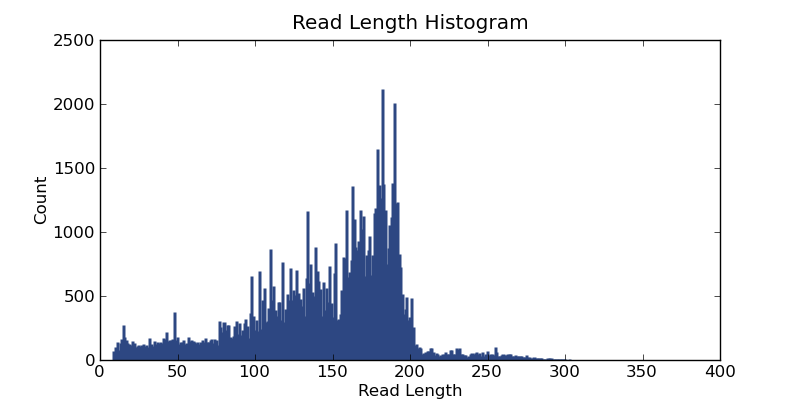
\includegraphics[width=\linewidth, keepaspectratio]{snp_calling/IonXpress_001_rawlib.read_len_histogram.png}
\end{center}
We will choose from one of the algorithms that are suited for longer reads, and
one of such algorithms is \texttt{map3}. To perform the read mapping we need to:
\begin{itemize}
  \item provide it with reference sequence (\texttt{-f \refRel})
  \item provide it with sequencing reads (\texttt{-r \mapReads.fastq})
  \item tell that sequencing reads are in \textit{FASTQ} format (\texttt{-i fastq})
  \item tell that we want alignment to be in compressed \textit{BAM} format(\texttt{-o 1})
  \item tell that we want output to be saved in a file named \texttt{\mapReads\_mapped.bam} (\texttt{-s \mapReads\_mapped.bam})
\end{itemize}
In linux terminal type:\\~\\
\tmap{\refRel}{\mapReads.fastq}{\mapReads\_mapped.bam}\\

We have obtained \textit{BAM} file. \textit{BAM} stands for \textbf{B}inary S\textbf{AM} file.
\textit{SAM}, in turn, stands for \textbf{S}equence \textbf{A}lignment/\textbf{M}ap format.

\subsubsection{\textit{BAM} file viewing and manipulation}
%Lekcija par bam failu
Let's find out what is in the first 20 lines of \textit{BAM} file using \texttt{samtools} and \texttt{head}:\\~\\
\texttt{samtools view \mapReads\_mapped.bam | head -n 20}\\

It is also possible to extract some specific region from the \textit{BAM} file with \texttt{samtools view}
by adding coordinates in form \texttt{chr\textit{N}:\textit{start}-\textit{end}} at the end of command:\\~\\
\texttt{samtools view \mapReads\_mapped.bam chr13:27925800-27925900}\\


%TODO aprakstīt katru no soļiem
To view \textit{BAM} file header, use 
\texttt{-H} option in \texttt{samtools view} command:\\~\\
\texttt{samtools view -H \mapReads\_mapped.bam}\\

As you can see, we have not defined our read group identifier (\texttt{ID:NOID})
and sample name (\texttt{SM:NOSM}). We can correct it using \texttt{samtools}
command \texttt{reheader}. It takes a \textit{BAM} header and \textit{BAM} file
as input. It replaces \textit{BAM} file's header with the provided header and 
outputs new \textit{BAM} file.

We will read our \textit{BAM} files header and modify it using \texttt{sed}
utility. The modified header will be given to \texttt{samtools reheader}
along with the original bam file. The output will be saved using \texttt{>}
operator:\\~\\
\reheader{\mapReads\_mapped.bam}{\mapReads\_mapped.reheaded.bam}\\

Alternatively, we could have simply defined the read group ID and sample name during mapping process,
using \texttt{tmap}'s option \texttt{-R}:\\~\\% with the complete tab delimited \texttt{RG} line of bam header:\\~\\
\tmapWithRG{\refRel}{\mapReads.fastq}{\mapReads\_mapped.reheaded.bam}\\

%\begin{framed}
%Note that the tab is denoted as \texttt{\textbackslash t} in our header line.
%\end{framed}

Detailed information about \textit{SAM/BAM} file format, see \url{http://samtools.github.io/hts-specs/SAMv1.pdf}.


We can use \texttt{samtools} command \texttt{tview} to view alignment in a
more human readable format. \texttt{tview} accepts only 
sorted and indexed \textit{BAM} files. Forunately, we can
do this easily using \texttt{samtools} commands 
\texttt{sort} and \texttt{index}:\\~\\
\texttt{samtools sort \mapReads\_mapped.reheaded.bam \mapReads\_mapped.reheaded.sorted}\\
\texttt{samtools index \mapReads\_mapped.reheaded.sorted.bam}\\

After sorting and indexing, we can view our \textit{BAM} file. In linux terminal type:\\~\\
\texttt{samtools tview \mapReads\_mapped.reheaded.sorted.bam \refRel}\\

Alignment will open in terminal. To get help on viewing alignment, type \texttt{?}.
Type \texttt{q} to quit viewer. A good place to view mapped reads and
test the viewer is \texttt{chr13:27925825}. To go to this position, type \texttt{g}
and enter this coordinate as it is shown.

%tview chr13:27925825
%region
%idxstats

\subsection{SNP calling}

To call SNPs we will use \texttt{samtools} and \texttt{bcftools}.
Using \texttt{samtools} we will generate our data in \textit{pileup} format which
is then accessed by \texttt{bcftools} to call SNPs.
\textit{Pileup} format is text based description of mapped bases at each position of reference sequence.
You can think of it as a vertical version of alignment viewing.
Variant callers need sorted by position \textit{BAM} file to successfuly detect variants
and we have already done that, so we can move to variant calling.
%To sort our \textit{BAM} file we will use \texttt{samtools}. In linux terminal type:\\~\\
%\sortbam{\mapReads\_mapped.reheaded.bam}{\mapReads\_mapped.reheaded.sorted.bam}\\

There are two choices of variant callers in \texttt{bcftools}:
\texttt{--consensus-caller} or \texttt{--multiallelic-caller}. \texttt{consensus-caller} is
older variant calling model and assumes only biallelic sites. It can miss somatic mutations.
\texttt{multiallelic-caller} does not have such an asumption and is more sensitive than \texttt{consensus-caller}.
%that the analyzed sample is biallelic and can miss somatic mutations. In contrast the \texttt{multiallelic-caller}
\texttt{multiallelic-caller} is recommended for most tasks, and we will also use it. For this tutorial, we will skip insertions/deletions: \\~\\
\samtoolssnp{\refRel}{\mapReads\_mapped.reheaded.sorted.bam}{\mapReads.bcftools\_snps.vcf}

%\subsection{Obtaining reference sequences}
%We begin our task by obtaining reference genome. We will download reference
%sequences in a seperate directory to avoid file cluttering. Let's make
%a new directory in our \texttt{\workDir}~named \texttt{\reseqDir}, and there we will create
%a seperate folder \texttt{\refDir} for our reference sequences:\\~\\
%\texttt{cd \textasciitilde}\\
%\texttt{cd \workDir}\\
%\texttt{mkdir \reseqDir}\\
%\texttt{cd \reseqDir}\\
%\texttt{mkdir \refDir}\\
%\texttt{cd \refDir}\\

%Our reference sequences can be accessed from a database made by
%University of California, Santa Cruz.
%The web address of the database is \url{http://genome.ucsc.edu/}.
%To find the necessary references sequences for chromosomes 1., 2. and 19.
%click on \texttt{Downloads} $\rightarrow$ \texttt{human} $\rightarrow$
%\texttt{Data set by chromosome}. Right click on \texttt{chr1.fa.gz}
%and \texttt{Copy link location}.
%Downloads->Human

\end{document}
